%!TEX root = /Users/rafaeldurelli/Dropbox/Artigos Elaborados/KDM propagation_2015/sbes_2015_kdm_propagation/sbes2015_kdm_propagation.tex
%


\begin{figure*}[t]
	\centering
	% Requires \usepackage{graphicx}
	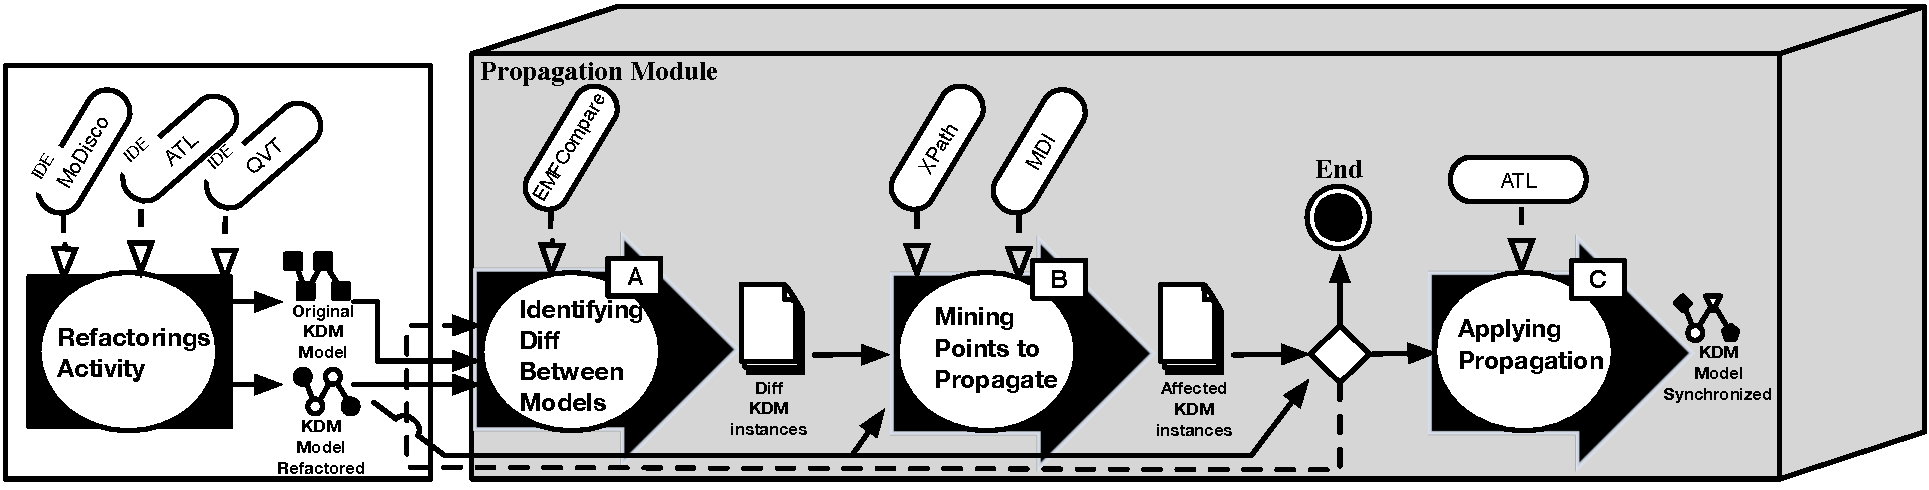
\includegraphics[scale=0.545]{figuras/ApproachLifeCicle2}
	\caption{A ``bird's eye'' View of our Approach.}
	\label{fig:approach}
\end{figure*}

In this section our approach is presented. It propagates changes, in a cascade way, throughout the KDM's levels during a refactoring. The intention is to keep the consistency/synchronization among all the KDM's views during a refactoring activities.
%
% in order to keep all the KDM views synchronized. The intention is to keep the consistency/synchronization among all the KDM's views during a refactoring activities. 
%
%In order to fulfill the limitation pointed out, we introduce a tool/approach, called Propagation-Aware Refactoring (PARef),  that aims propagating changes throughout all the KDM's levels during a refactoring in order to keep all the views synchronized. The intention is to keep the consistency among all the KDM's views during refactoring activities.
%
Figure~\ref{fig:approach} shows the workflow of our approach. It contains three steps, [A], [B], and [C] all contained into the gray box. Outside of our approach there is the \textit{Refactoring Activity}, see the white rectangle. This activity is a normal and conventional model refactoring activity - this activity is out of scope of our approach - is responsibility of the software modernizer to develop or reuse any model refactorings (in ATL, ETL, QVT, etc) and apply them into a KDM model. %In this phase, a number of KDM model elements can be modified, created or removed. 

After that, the first step, [A] is trigged then a diff between the refactored KDM instance and the original KDM instance (the instance before one applies a KDM refactoring) is performed. The output of this diff is a list that contains all KDM model instance involved during the KDM refactoring. %Further our two-steps approach starts.  

From this point onward, the step [B], called \textit{Mining Points to Perform the Propagation} gathers all the KDM elements that need to be updated/synchronized as a result of a refactoring. %This step uses the list that was obtained from the diff between the refactored KDM and original KDM instance (step [A]) as input. 
This step runs a depth-first search algorithm (from here on in \textbf{M}ining \textbf{D}ependents \textbf{I}dentification Algorithm - MDI Algorithm). This algorithm uses as input the list that was obtained from the diff between the refactored KDM and original KDM instance (step [A]).
It also uses the refactored KDM instance to generate as output all KDM instances that possesses dependencies with the elements to be refactored. 

The third step [C], called \textit{Applying Propagation}, applies all the changes/updates in the KDM instance. The inputs for this step are the meta-class instances to be changed (provided in step [B]) and the output is the refactored KDM instance.

An important point is that this three-step sequence is repeated in a cascade way until no more elements need to be updated, which is represented by the dotted line that goes back to the first step or forward to the final state. This cycle is necessary because the refactored KDM instance can still require propagations in other elements/views, so, each cycle concentrates just on the next level. The stop condition is when the mining algorithm returns an empty set, indicating that there are no more elements that depend on the modified ones.

The step [A], is technically supported by the framework EMF Compare as it provides comparison and merge facility for any kind of model. Herein EMF Compare was reused and extended to compare instances of KDM models. The step [B], is technically supported by an \textit{Identification Engine} whose the core is our MDI Algorithm along with a set of queries that are performed over a KDM model. %The \textit{Identification of the Points To Be Propagated} is easier to be done after the refactoring and the after performing the diff between , because it is possible to detect the already changed elements making a diff between the source and refactored model. %When the identification process should be done before the refactoring application, all the model elements involved in the refactoring need to be extracted and passed as parameters to the Identification Engine. This will require more implementation effort.

The step [C] is technically supported by a \textit{Propagation Engine}, whose core is a set of pre-defined transformation rules devised with ATL that works in cascade way. All the transformation rules act as a chain of transformations that are executed together in order to update/propagate all the changes throughout KDM's views. More details on each step are provided in the next sections.


%This approach ensures that when a change/refactoring is performed in any KDM's level, it is correctly propagated to the affected KDM's levels and vice versa. So it make certain that the consistency between the KDM's levels when they are refactored. Our approach is called Propagation-Aware Refactoring (PARef) and it is split into three steps, which are depicted by its corresponding letters and tittle in Figure~\ref{fig:approach}. 

%According to the literature, there are two possibilities to perform propagation in models (colocar ref). One possibility is to mark the modifications on the source KDM's model without actually commiting them until the end of the transformation, so that expression evaluation can occur on the original source KDM's model by ignoring the modifications. Another possibility is to first compute the set of basic operations to perform, storing this set in an external artifact representation and then apply all the changes at once. Our approach follows the second possibility and it is divided in three steps, which are depicted by its corresponding letters and tittle in Figure~\ref{fig:approach}.


%In step [A], \textit{Apply Refactoring}, here the software modernizer has to choose an appropriate refactoring to be applied into the KDM. In this step, new metaclasses can be created, updated, and removed. Also it is necessary to gather all the needed parameters for applying the refactoring. %that the software modernizer inputs all the needs parameters for applying the refactoring is gathered.  %The most frequent modification to the KDM instances in this scenario will be, intuitively, creating new metaclasses. However, updating existing metaclasses with their relationship will be frequent as well. In simpler cases, updating means changing properties of existing metaclasses. In more complex cases, updating means removing metaclasses and replacing them with new and refactored ones. This step uses model-to-model (M2M) transformation language to perform the refactorings.

%In the step [B], \textit{Mine Affected Metaclasses}, we developed a mechanism which shows all metaclasses that need to be updated/propagated after applying any changes/refactoring. These metaclasses are those that have some dependence on the metaclass to be modified by the refactoring. This step is totally based on a set of queries that works on a KDM instance. In addition, this step uses depth-first search algorithm\footnote{From here on in Dependents Identification Algorithm (DI Algorithm)} to identify all affected metaclasses along with a set of queries. 

%In step [C], \textit{Propagate Changes}, involves updating the elements identified in the step [B].  As in step [A], in this step we also have used M2M to update/propagate all KDM's instances. 

\subsection{Identifying Diff Between Models}

%The problem of model diff is intrinsically complex. For instance, if a ClassUnit C is deleted, its transitive parts and attached associations are typically also deleted. So, computing the difference results in a large number of detail changes that might be complex to implement from scratch. 

We have integrated  EMF Compare\footnote{https://www.eclipse.org/emf/compare/} with our plug-ing because it is a framework that can easily reuse and extend to compare instances of any models, in our case KDM models. %EMF Compare also was designed with scalability in mind in order to support comparisons of large fragmented models.

To start this step, our plug-ing needs two instance of KDM as input: i) the refactored one (left side), and ii) the original (right side). Our plug-ing analyses, whether the KDM elements are equal or if they present differences (for example, the name of the class has been changed from Class1 to ClassX, or a class has been moved from a Package to another Package, etc). Then, our plug-ing iterates over all of our KDM elements, be they unmatched (only one side has this object), couples (two of the three sides contain this object) and compute any difference that may appear between the sides. 
For example, a KDM element that is only on one side of the comparison is a KDM element that has been added, or deleted. But a couple might also represent a deletion: during three way comparisons, if we have an KDM element in the common ancestor (origin) and in the left side, but not in the right side, then it has been deleted from the right side version. The output of this step is a list that contains all KDM model elements involved during the KDM refactoring. 

\subsection{Mining Points to Perform the Propagation} % (fold)
\label{sub:mine_affected_metaclasses}

The step [B] starts with MDI Algorithm to identify all affected meta-classes along with a set of queries. The MDI Algorithm recognizes all meta-classes and its relationships that use somehow the meta-class(es) that were refactored. As input our MDI Algorithm uses the list obtained from the Step [A]. For example, in the case of the refactoring \textit{Move Class} the list would contains a Package and a set of ClassUnits that were moved. Further, our MDI Algorithm uses a set of queries that are performed on the KDM's instance to mine all the affected/linked meta-classes. All the queries were created using XPath. We have decided to use XPath because it is a well-know and well-documented language. 

%Concerning the refactoring \textit{Move Class} the engineer should specify a set of classes that no longer are contained into a package \texttt{View}. These classes should be allocated into the package \texttt{Model}. 
%Considering the refactoring \textit{Move Class}, three elements (\texttt{Student}, \texttt{Instructor}, and their package) need to be investigated throughout the KDM's instance in order to identify which other metaclasses can be affected. 

Firstly a query must be executed to get the root element in KDM. This query is represented as the first statement in Figure~\ref{fig:queriesXPath}, see line 1 - it is used to return an instance of the meta-class \texttt{Segment}. The returned Segment, as well as all KDM's views are gathered by the other queries presented in Figure~\ref{fig:queriesXPath} lines 2 to 5. The returned elements of these queries are used as input in our MDI Algorithm as all the the list obtained from the Step [A].

\begin{figure}[h]
	\centering
	% Requires \usepackage{graphicx}
	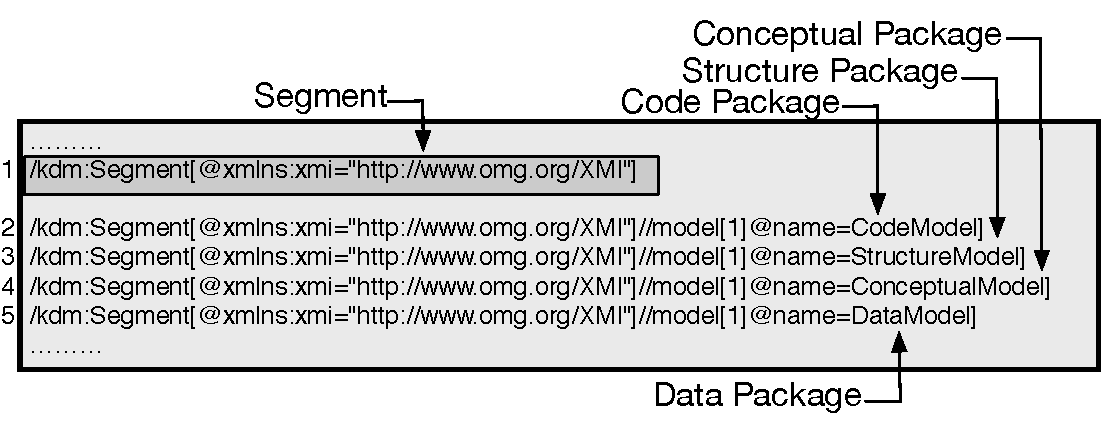
\includegraphics[scale=0.479]{figuras/queiresANDATLSBESNew}
	\caption{Xpath used to return the KDM's elements.}
	\label{fig:queriesXPath}
\end{figure}


\begin{algorithm}[h]
     \SetAlgoLined
     \KwIn{DFS (G, u, eL) where G is a KDM's instance, u is the initial meta-class, i.e., Segment, and eL is a set of elements to verify}
     \KwOut{A collection of affected meta-classes}
     \Begin{
     \ForEach{$outgoing$ edge e = (u, v) of u} {
	\If{vertex v as has not been visited }{
			\If{vertex v contain implementation = true }{
				
				\ForEach{$implementations$ element}{
				verify all elements in implementation
				}
				Mark vertex v as visited (via edge e).
				Recursively call DFS (G, v).
			}
			
				}				
			}		
	
	}
     \caption{MDI(G,u) - Mining Dependents Identification Algorithm.}
     \label{alg:death1}
   \end{algorithm}

Algorithm~\ref{alg:death1} depicts the MDI Algorithm that is used to mine all the affected meta-classes. %It takes as input a KDM's instance, a \texttt{Segment}, and a set of elements that were refactored in Step [A] (e.g., for the refactoring \textit{Move Class} three affected elements - \texttt{Student}, \texttt{Instructor}, and their package). %A diagram of how our DI Algorithm works is shown in Figure~\ref{fig:algWorks2}. Each node represents a metaclass and the edges represent the relationship among the metaclasses - the node A represents the \texttt{Segment} and K, H, E and B illustrate \texttt{CodeModel}, \texttt{StructureModel}, \texttt{ConceptualModel}, and \texttt{DataModel}, respectively. 
%
The algorithm works as follows: first it is necessary to pick a starting point, i.e., the meta-class \texttt{Segment}. Visit the \texttt{Segment}, push it onto a stack, and mark it as visited. Then it is necessary to go to the next meta-class that is unvisited, verify if it has an association named \texttt{implementation}. If so, it verifies if this association contains references to any element's used in the refactoring, if so - push it on the stack, and mark it. This continues until the algorithm reaches the last meta-class. Then the MDI Algorithm checks to see if the \texttt{Segment} has any unvisited adjacent meta-class. If it does not, then it is necessary to pop it off the stack and check the next meta-class. If the algorithm finds one (unvisited meta-class), it starts visiting adjacent meta-classes until there are no more, check for more unvisited adjacent meta-classes, and continue the process always verifying the association named \texttt{implementation}. When the algorithm finally reach the last meta-class on the stack and there are no more adjacent, unvisited meta-classes that contains the association \texttt{implementation} without check, our algorithm should create a list of all affected meta-classes that is further used to propagated all changes throughout the KDM levels. 
%
%
%
%
%
%
%
%
%

%\begin{figure}
%	\centering
	% Requires \usepackage{graphicx}
%	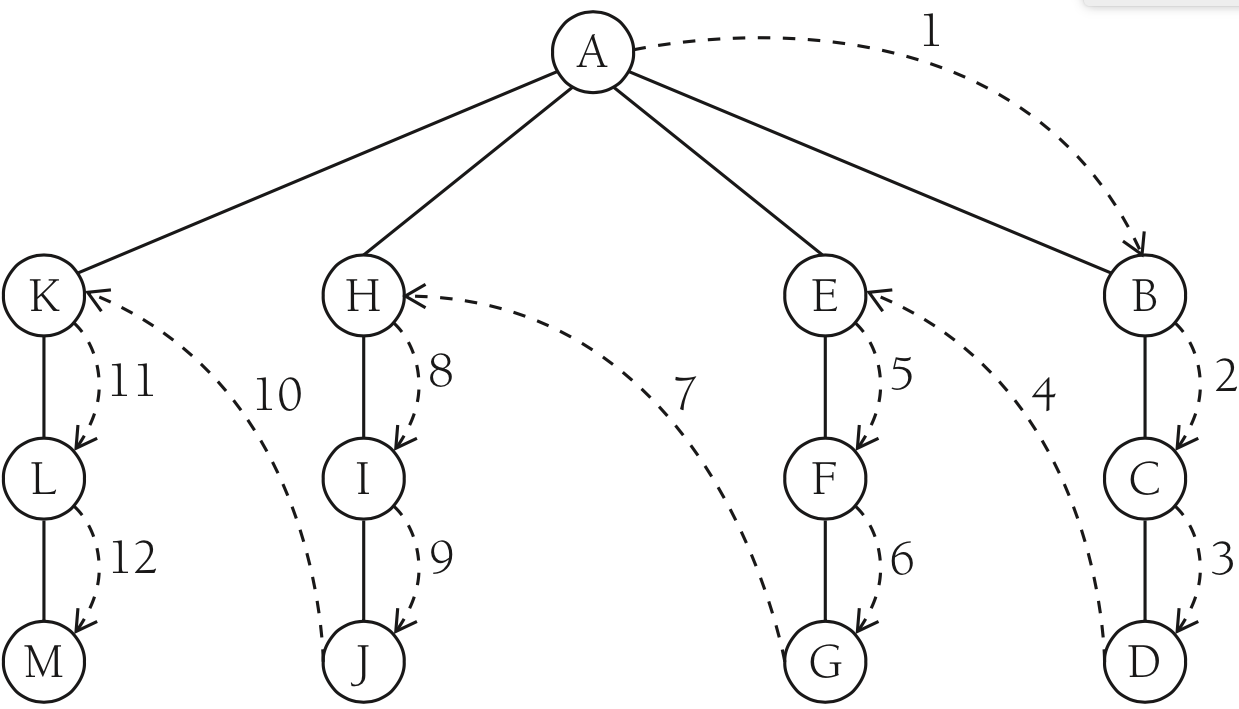
\includegraphics[scale=0.2]{figuras/algWorks2}
%	\caption{Depth-First Search.}
%	\label{fig:algWorks2}
%\end{figure}






%As can be visualized, a stack is used to store all affected elements, see Algorithm~\ref{alg:death1} line 2, \ding{182}. In line 3 a generic KDM element is defined. While \textit{seg} is non-empty, a node is chosen for expansion (line 4). %For fact edges, the dependency of the edge on the particular fact that caused its creation is then recorded (lines 14- 16)





%\begin{algorithm}[h]
%     \SetAlgoLined
%     \KwIn{KDMEntity kdmElement, Segment segment, KDMModel model}
%     \KwOut{All affected metaclasses}
%     \Begin{
%   $ Stack stack \longleftarrow \{\}$\;
%   KDMEntity elementToVerify\;
%     \ForEach{$seg$ in $segment$} {
%	\eIf{seg.getOwnedElements() != null}{
%			\If{seg.getNextSiblind() != null}{
%				$elementToVerify \longleftarrow seg.getNextSiblind()$\;
%		\If{\ding{182} isAffected(elementToVerify, kdmElement, model)}{
%					stack.push(elementToVerify)\;
%					$seg \longleftarrow  seg.getFirstChild()$\;
%				}				
%			}		
%	
%	}{ $seg \longleftarrow seg.getNextSiblind()$\;
%		\If{seg = null \&\& stack.isEmpty()}{
%			// return to the parent's level
%		}
%	}
%     }
%	\ding{184} \Return{stack}
%     }
%     \caption{Depth-First Search Algorithm.}
%     \label{alg:death1}
%   \end{algorithm}
%
%\begin{algorithm}[h]
%     \SetAlgoLined
%     \KwIn{KDMEntity kdmElement, KDMModel model, KDMEntity e}
%     \KwOut{true or false}
%     \Begin{
%     	\If{ (e = AbstractUIElement) or (e = AbstractStructureElement) or (e = BuildResource) or (e = AbstractPlatformElement) or (e = AbstractConceptualElement) or (e = AbstractEventElement)
%				} {
%					     \ForEach{$elements$ in $e.getImplementation()$} {
%					\If{ elements = ele} {
%					\Return{true}
%					}
%					}				
%				}
%\uElseIf{ e = AbstractDataElement
%				} {
%					     \ForEach{$elements$ in $elementToV.getDataRelation()$} {
%					\If{ elements = elementToVerify} {
%					\Return{true}
%					}
%					}				
%				}
%	...
%     }
%     \caption{isAffected Algorithm}
%     \label{alg:death}
%   \end{algorithm}

%As every element, except the Segment, is connected somehow it is necessary to iterate throughout them, line 4 of Algorithm~\ref{alg:death} illustrates this iteration. After, the method \texttt{isAffected(...)} is called to verify if the element is affected.  If the condition in line 8 evaluates to true, then the element is pushed into the stack defined in line 2. Finally, in line 20 the stack is returned with all affected elements, see Algorithm~\ref{alg:death} \ding{184}. 



\subsection{Applying Propagation} % (fold)
\label{sub:apply_refactoring}

This step objectives to effectively perform in a cascade way all the changes/updates in the KDM model. 
%
%This step is a decoupled module that can be coupled to existing refactorings. In this way, existing users can write KDM refactorings in ATL without worrying about the change propagation, which is a time-consuming and error-prone task. 
The only task is to provide for this step all the parameters it needs to conduct the propagation. By means of our plug-in these parameters are identified automatically in Step [B] and are used in Step [C]. 
%
%
 %all propagations regarding an specific refactoring, e.g., \textit{Move Class}, are implemented. 
Differently from step [A], where the modernizer has to define a set of model transformations rules to perform the model refactoring, here a set of generic and pre-established model transformations (written in ATL) are used. More specifically, the difference is that in Step [A], the modernizer can either create or reuse a KDM refactoring, otherwise in Step [C] all rules were beforehand defined to perform the propagation of changes (in a cascade way) after the application of a KDM refactoring. In addition, these ATL rules (the propagations) require a set of  \textit{mininum} parameters that should be informed before realize all the propagations. As already mentioned these parameters are the output from Step [B], which is a list containing all KDM affected instances. 

In order to bound these parameters along with the output of Step [B] our approach performs a static analysis (parsing) of all generic ATL rules and identifies places that must be replaced in with the Step [B]'s output (KDM affected instances), i.e, all the places where parameters are needed. This is particularly necessary in our approach because ATL does not enforce type correctness, hence rules written in ATL may be ill-typed. Moreover, the creation of a suitable propagation %in this step 
requires precise parameters (meta-classes) informations. It is important to highlight that this static analysis is done totally automatically and transparently by means of our Eclipse plug-in. The aim is having a decouple module of KDM propagation as simple as possible to facilitate the integration with any refactoring defined in ATL in the context of KDM model and also to promote the reuse. Therefore, the software modernizer does not have to worry about devising the propagation of changes, which usually is harder than just the creating of a KDM refactoring. 
%
In addition, if the static analysis detect errors, the software modernizer is required to fix and inform the correct parameters, otherwise, all changes are propagated in all KDM levels automatically/transparently  


Figure~\ref{fig:ATLPropagation} shows a code snippet written in ATL that is used to propagate the changes. Due space limitation the whole ATL it is not presented. Note that all strings, \textbf{`\#parameter'}, are changed during the static analysis along with the step [B]'s output. As can be seen, there are three rules - each of them is used to propagated the change in a specific KDM package, respectively. The first rule is responsible to propagate the changes throughout the \texttt{Structure View}, see lines 24 to 32. In line 26 the source pattern of the rules is defined by using OCL guard stating the layers to be matched. After, is defined a target pattern (lines 29 -31) which is used to compute the \texttt{density} of an \texttt{AggregationRelationship} after the application of a refactoring, i.e, \textit{Move Class}.

\begin{figure}[h]	
	\centering
	% Requires \usepackage{graphicx}
	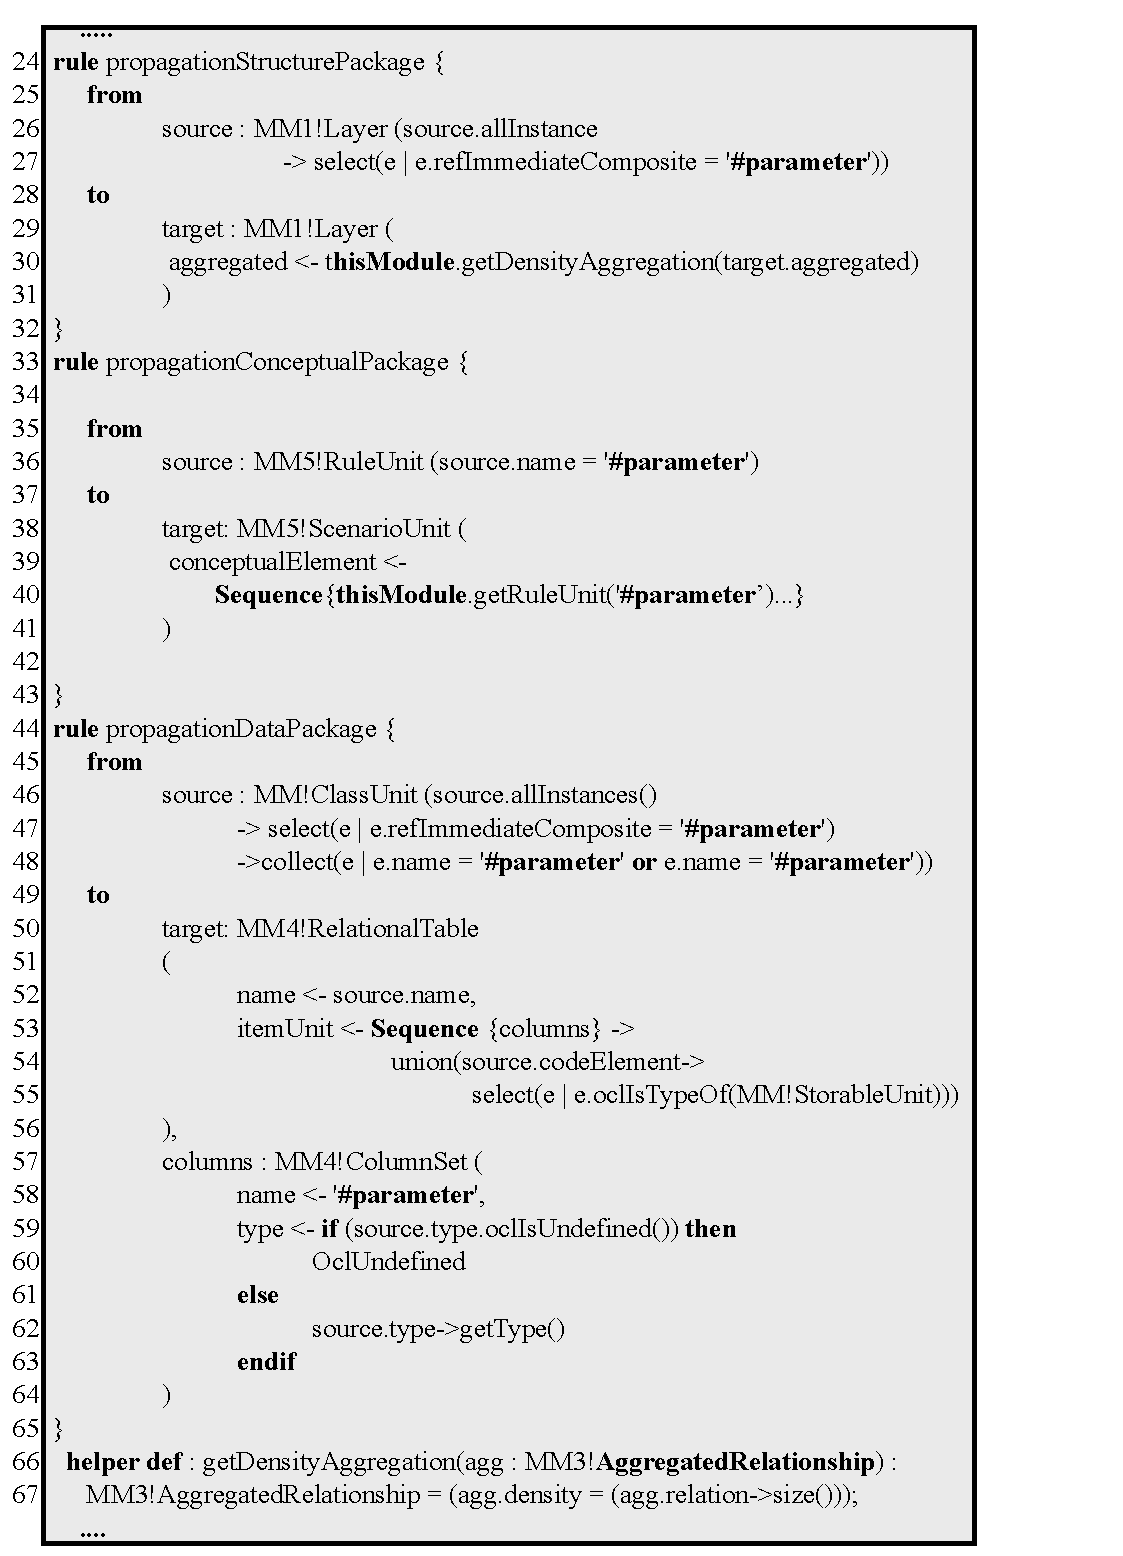
\includegraphics[scale=0.516]{figuras/ATLPRopagationSBESFormatted}
	\caption{Snippet of ATL to execute the propagation in cascade.}
	\label{fig:ATLPropagation}
\end{figure}

If the \textit{Move Classes} refactoring is applied to transfer the classes to a package to another as illustrated in the Section~\ref{sec:running_example}, a natural propagation is to transfer the business rule related to the moved classes to another scenario that represent the target package. A chunk of propagation is defined in the second rule (lines 33 to 43) - it can be used to propagate the changes throughout the \texttt{Conceptual View}.
%
%The rule defined in lines 33 to 43 propagates the changes throughout the \texttt{Conceptual Package}. If the \textit{Move Classes} refactoring is applied to transfer the class C1 to package P2, a natural propagation is to transfer the business rule B1 to another scenario.
%
%
% For instance, Line 36 shows the specific propagation that is ne the \texttt{RuleUnit 1.1} that is associated with \texttt{Instructor} should also be moved to corresponding scenario, i.e, the scenario that is associated with the package that contains now the class \texttt{Instructor} - \texttt{ScenarioUnit 3}. 
%
 Finally, the rule defined in lines 44 - 65 propagates the change to the \texttt{Data View}. For each new \texttt{ClassUnit} instance a \texttt{RelationalTable} instance has to be created - their names have to correspond. The \texttt{itemUnit} %(a collection that contains \texttt{ColumnSet}) 
reference set has to contain all \texttt{ColumnSet} that have been created for each \texttt{StorableUnit} (meta-class that represent all the attributes that a class holds) as well as its types.

%In the step [C] all the changes, that where resulted by the refactoring  performed in step [b] need be propagate into all KDM's levels/package.  

%The correctness of our Propagation Engine mainly relies on the compliance of the transformation result, which in turn can be ensured by showing that the transformation produces a consistent KDM model. Thus, it is important to support the consistency among all KDM views. To this end, we consider static consistency checks.

Although we have used a simple KDM refactoring as example (\textit{Move Class}), by observing both Figure~\ref{fig:ATLRefactoring} and Figure~\ref{fig:ATLPropagation} it is fairly evident that the refactoring itself usually is less complex/verbose to devise than the Propagation Engine, i.e., a set of pre-defined rules to propagate the changes in KDM views tend to be more complex/verbose than KDM refactorings. Therefore, we argue to provide a module that can be plugged over existing KDM refactorings in order to propagate the changes can assist the software modernizer.

% Due space limitation the whole ATL that is used to promote the propagation is not shown - but by observing both ATL that the rules to perform the propagation are much more complex. 
